\documentclass{article}

\usepackage{amsmath}
\usepackage{tikz}

\begin{document}

    \begin{center}
        \textbf{BILANGAN KOMPLEKS}
    \end{center}

    Bilangan Kompleks adalah bilangan yang dapat direpresentasikan sebagai \( x + iy \), dimana $x$ dan $y$ adalah bilangan real ($R$) dan $i$ adalah suatu bilangan imaginer dimana \( i = \sqrt{-1} \) dan \( i^2 = -1 \).\\

    Bilangan Kompleks biasanya ditulis dalam bentuk:
    \begin{align}
        x = x + iy
    \end{align}

    \>dimana,\\
    - $x$ adalah bagian $Re(z)$, dan\\
    - $y$ adalah bagian $Im(z)$.\\

    Contoh:
    \begin{align}
        z & = 6 + \sqrt{-16} 
        \nonumber\\
        & = 6 + \sqrt{-1} \times \sqrt{16}
        \nonumber\\
        & = 6 + i \times 4
        \nonumber\\
        & = 6 + 4i
    \end{align}

    maka:\\
    -   $Re(z) = 6$, dan\\
    -   $Im(z) = 4$.\\\\

    \begin{center}
        \textbf{Notasi Bilangan Kompleks}
    \end{center}

    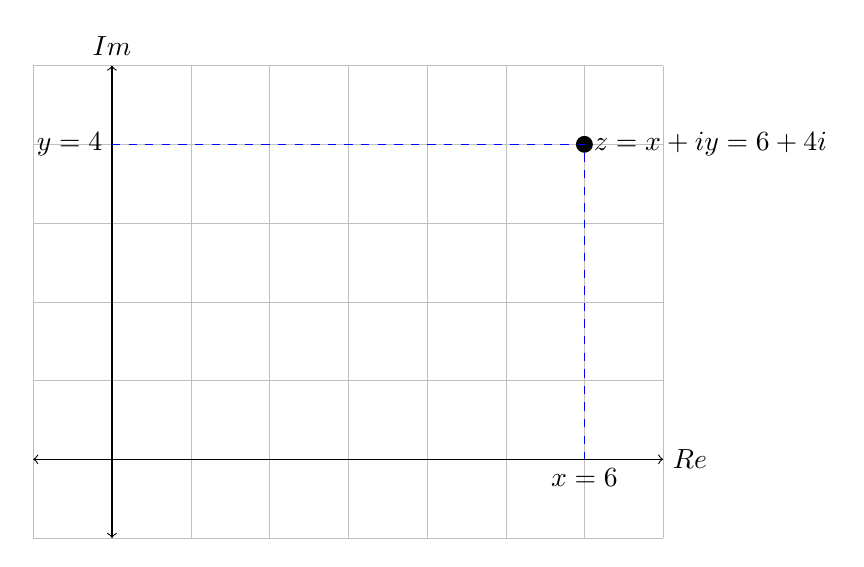
\begin{tikzpicture}
        \draw [ultra thin, lightgray] (-1,-1) grid (7,5);
        \draw [<->] (-1, 0) -- (7, 0) node[right] {$Re$};
        \draw [<->] (0, -1) -- (0, 5) node[above] {$Im$};
        \draw [black, fill = black] (6,4) circle [radius = 1 mm]
            node[black, right] {$ z = x + iy = 6 + 4i $};
        \draw [blue, dashed] (0,4) node[black, left] {$ y = 4 $}
            -| (6,0) node[black, below] {$ x = 6 $};
    \end{tikzpicture}
    \\ \\ \\ \\

    Misal $ z_1 = ( x_1 , y_1 )  $ dan $ z_2 = ( x_2 , y_2 ) $, maka berlaku:

    \begin{align}
            z_1 + z_2   & = ( x_1 \;,\; y_1 ) + ( x_2 \;,\; y_2 )
            \nonumber\\
            & = ( x_1 + x_2 \;,\; y_1 + y_2 )
            \\\nonumber\\
            z_1 \cdot z_2   & = ( x_1 \;,\; y_1 ) \cdot ( x_2 \;,\; y_2 )
                            \nonumber\\
                            & = ( x_1 x_2 - y_1 y_2 \;,\; x_1 y_2 + x_2 y_1 )
                            \\\nonumber\\
            a \cdot z_1 & = a \cdot ( x_1 \;,\; y_1 )
                        \nonumber\\
                        & = ( ax_1 \;,\; ay_1 )
    \end{align}
    \\ \\ \\ \\

    \begin{center}
        \textbf{Modulus Bilangan Kompleks}
    \end{center}

    Modulus atau nilai absolut bilangan kompleks $ z = x + iy $, didefinisikan sebagai bilangan real tidak negatif yang merupakan panjang vektor posisi dari $z$ (jarak antara $z$ dengan pusat sumbu).
    \\ \\

    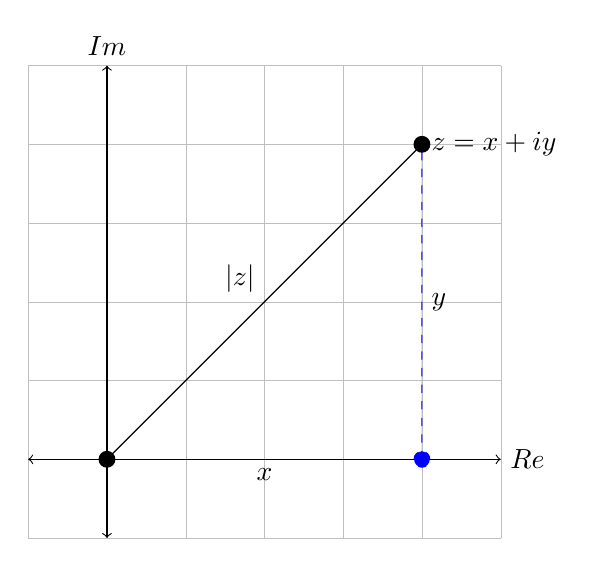
\begin{tikzpicture}
        \draw [ultra thin, lightgray] (-1,-1) grid (5,5);
        \draw [<->] (-1, 0) -- (5, 0) node[right] {$Re$};
        \draw [<->] (0, -1) -- (0, 5) node[above] {$Im$};
        \draw [black, fill = black] (4,4) circle [radius = 1 mm] 
            node[black, right] {$ z = x + iy $};
        \draw [black, fill = black] (0,0) circle [radius = 1 mm] -- (4,4);
        \draw [dashed, blue, fill = blue] (4,0) circle [radius = 1 mm] -- (4,4);
        \draw (2,2) node[above, anchor=south east, black] {$|z|$};
        \draw (4,2) node[right, black] {$y$};
        \draw (2,0) node[below, black] {$x$};
    \end{tikzpicture}
    \\ \\

    \begin{align}
        |z|         &= \sqrt{x^2+y^2}
        \\\nonumber\\
        |z_1 - z_2| &= \sqrt{(x_1-x_2)^2 + (y_1-y_2)^2}
    \end{align}
    \\ \\

    Sifat Modulus
    \begin{align}
        \bigg | \frac{z_1}{z_2} \bigg | &= \frac{|z_1|}{|z_2|}
        \\\nonumber\\
        |z_1 z_2|                       &= |z_1| \cdot |z_2|
    \end{align}
    \\ \\ \\ \\

    \begin{center}
        \textbf{Sekawan/\textit{Konjugate} Bilangan Kompleks}
    \end{center}

    Misalkan $ z = x + iy $, sekawan dari $z$ (notasi = $\overline{z}$) adalah pencerminan dari $z$ terhadap sumbu real ($R$).
    \\ \\ 

    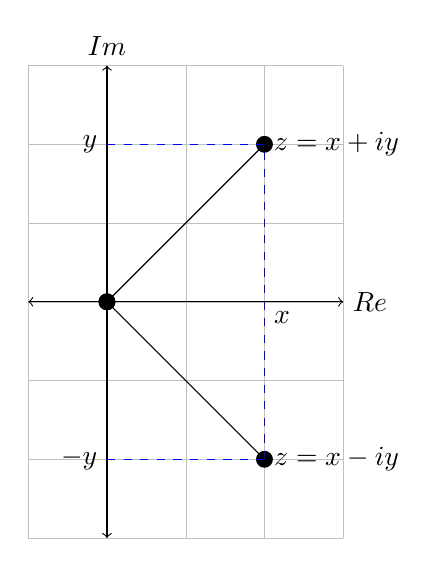
\begin{tikzpicture}
        \draw [ultra thin, lightgray] (-1,-3) grid (3,3);
        \draw [<->] (-1, 0) -- (3, 0) node[right] {$Re$};
        \draw [<->] (0, -3) -- (0, 3) node[above] {$Im$};
        \draw [black, fill = black] (2,2) circle [radius = 1 mm] 
            node[black, right] {$ z = x + iy $};
        \draw [black, fill = black] (2,-2) circle [radius = 1 mm] 
            node[black, right] {$ z = x - iy $};
        \draw [black, fill = black] (0,0) circle [radius = 1 mm] -- (2,2);
        \draw [black, fill = black] (0,0) circle [radius = 1 mm] -- (2,-2);
        \draw [dashed, blue] (2,-2) -- (2,2);
        \draw [dashed, blue] (0,2) node[left, black] {$y$} -- (2,2);
        \draw [dashed, blue] (0,-2) node[left, black] {$-y$} -- (2,-2);
        \draw (2,0) node[below right, black] {$x$};
    \end{tikzpicture}
    \\ \\ \\ \\

    Sifat Sekawan/\textit{Konjugate}:
    \begin{itemize}
        \item $\overline{z_1 + z_2} = \overline{z_1} + \overline{z_2}$
        \item $\overline{z_1 z_2} = \overline{z_1} \cdot \overline{z_2}$
        \item $|z| = \overline{z}$
        \item $\overline{zz} = |z|^2$
        \item $Re(z) = \dfrac{z+z}{2}$\\ \\
            $Im(z) = \dfrac{z-z}{2i}$
    \end{itemize}

    \end{document}